\documentclass[margin=3mm]{standalone}
\usepackage{tikz}
\usepackage{pgfplots}
\pgfplotsset{compat=1.16}
\begin{document}
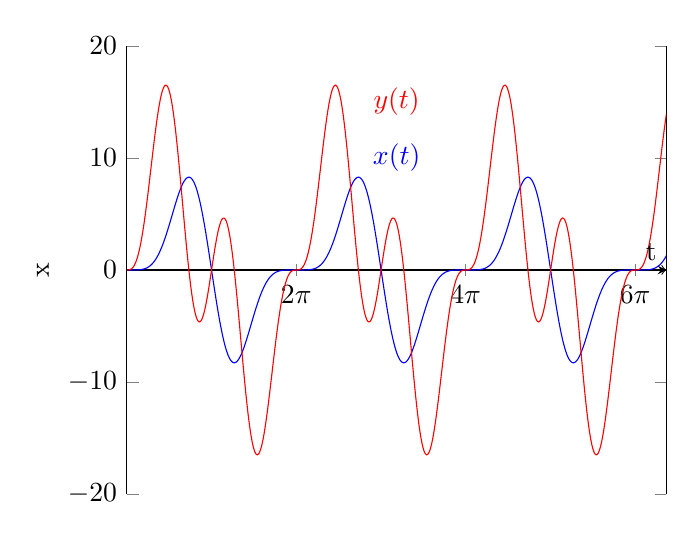
\begin{tikzpicture}
\begin{axis}[
	xmin = 0,	
	xmax = 20,
	axis x line = middle,
	%axis y line = center,
	ymin = -20,
	ymax = 20,
	ylabel=x,
	xlabel=t,
	xtick={6.28,12.56,18.84},
	xticklabels={$2 \pi$, $4 \pi$, $6 \pi$},
	domain=0:20
]
\draw [->] (0,0) -- (20,0);
\addplot [color=blue, samples=500] plot ({\x},{5*sin(deg(\x)) - 4 * sin(2* deg(\x)) + sin(3 * deg(\x))});
\addplot [color=red, samples=500] plot ({\x},{10*sin(deg(\x)) + 4 * sin(2* deg(\x)) - 6 * sin(3 * deg(\x))});
\draw [color=red] (10,15) node {$y(t)$};
\draw [color=blue] (10,10) node {$x(t)$};
\end{axis}
\end{tikzpicture}
\end{document}